% Created by tikzDevice version 0.12.6 on 2025-04-17 10:36:57
% !TEX encoding = UTF-8 Unicode
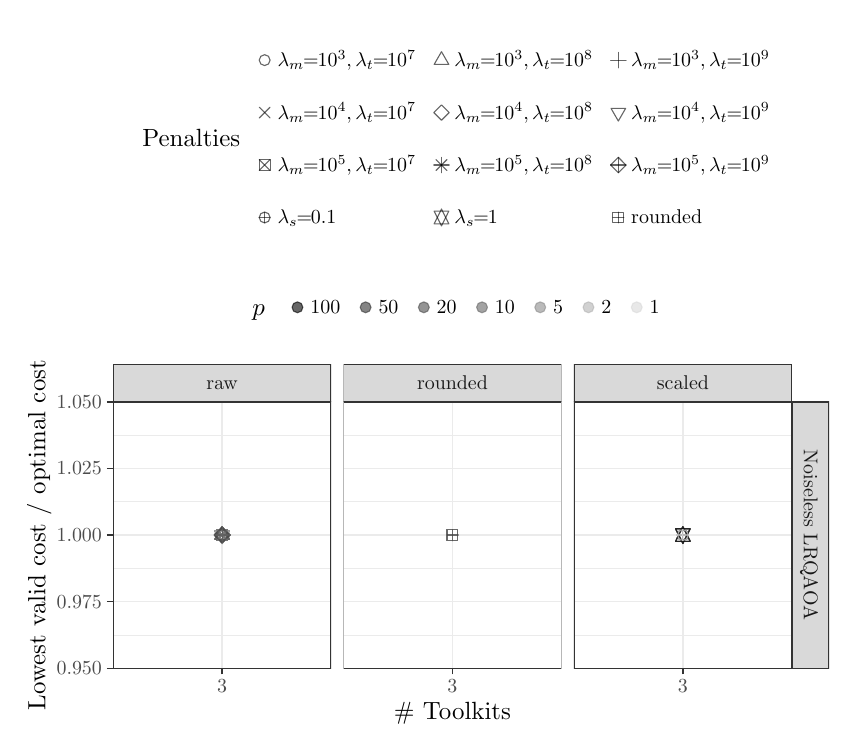
\begin{tikzpicture}[x=1pt,y=1pt]
\definecolor{fillColor}{RGB}{255,255,255}
\path[use as bounding box,fill=fillColor,fill opacity=0.00] (0,0) rectangle (289.58,251.81);
\begin{scope}
\path[clip] (  0.00,  0.00) rectangle (289.58,251.81);
\definecolor{drawColor}{RGB}{255,255,255}
\definecolor{fillColor}{RGB}{255,255,255}

\path[draw=drawColor,line width= 0.5pt,line join=round,line cap=round,fill=fillColor] (  0.00,  0.00) rectangle (289.58,251.81);
\end{scope}
\begin{scope}
\path[clip] ( 30.88, 20.35) rectangle (109.63,116.59);
\definecolor{fillColor}{RGB}{255,255,255}

\path[fill=fillColor] ( 30.88, 20.35) rectangle (109.63,116.59);
\definecolor{drawColor}{gray}{0.92}

\path[draw=drawColor,line width= 0.2pt,line join=round] ( 30.88, 32.38) --
	(109.63, 32.38);

\path[draw=drawColor,line width= 0.2pt,line join=round] ( 30.88, 56.44) --
	(109.63, 56.44);

\path[draw=drawColor,line width= 0.2pt,line join=round] ( 30.88, 80.50) --
	(109.63, 80.50);

\path[draw=drawColor,line width= 0.2pt,line join=round] ( 30.88,104.56) --
	(109.63,104.56);

\path[draw=drawColor,line width= 0.5pt,line join=round] ( 30.88, 20.35) --
	(109.63, 20.35);

\path[draw=drawColor,line width= 0.5pt,line join=round] ( 30.88, 44.41) --
	(109.63, 44.41);

\path[draw=drawColor,line width= 0.5pt,line join=round] ( 30.88, 68.47) --
	(109.63, 68.47);

\path[draw=drawColor,line width= 0.5pt,line join=round] ( 30.88, 92.53) --
	(109.63, 92.53);

\path[draw=drawColor,line width= 0.5pt,line join=round] ( 30.88,116.59) --
	(109.63,116.59);

\path[draw=drawColor,line width= 0.5pt,line join=round] ( 70.25, 20.35) --
	( 70.25,116.59);
\definecolor{drawColor}{RGB}{77,77,77}

\path[draw=drawColor,draw opacity=0.60,line width= 0.4pt,line join=round,line cap=round] ( 67.48, 68.47) -- ( 73.03, 68.47);

\path[draw=drawColor,draw opacity=0.60,line width= 0.4pt,line join=round,line cap=round] ( 70.25, 65.70) -- ( 70.25, 71.25);

\path[draw=drawColor,draw opacity=0.60,line width= 0.4pt,line join=round,line cap=round] ( 67.48, 68.47) --
	( 70.25, 71.25) --
	( 73.03, 68.47) --
	( 70.25, 65.70) --
	cycle;
\definecolor{drawColor}{RGB}{0,0,0}

\path[draw=drawColor,draw opacity=0.60,line width= 0.4pt,line join=round,line cap=round] ( 70.25, 65.42) --
	( 72.89, 70.00) --
	( 67.61, 70.00) --
	cycle;
\definecolor{drawColor}{RGB}{140,140,140}

\path[draw=drawColor,draw opacity=0.60,line width= 0.4pt,line join=round,line cap=round] ( 70.25, 68.47) circle (  1.96);
\definecolor{drawColor}{RGB}{102,102,102}

\path[draw=drawColor,draw opacity=0.60,line width= 0.4pt,line join=round,line cap=round] ( 70.25, 65.42) --
	( 72.89, 70.00) --
	( 67.61, 70.00) --
	cycle;
\definecolor{drawColor}{RGB}{77,77,77}

\path[draw=drawColor,draw opacity=0.60,line width= 0.4pt,line join=round,line cap=round] ( 70.25, 71.52) --
	( 72.89, 66.95) --
	( 67.61, 66.95) --
	cycle;
\definecolor{drawColor}{RGB}{51,51,51}

\path[draw=drawColor,draw opacity=0.60,line width= 0.4pt,line join=round,line cap=round] ( 67.48, 68.47) -- ( 73.03, 68.47);

\path[draw=drawColor,draw opacity=0.60,line width= 0.4pt,line join=round,line cap=round] ( 70.25, 65.70) -- ( 70.25, 71.25);
\definecolor{drawColor}{RGB}{217,217,217}

\path[draw=drawColor,draw opacity=0.60,line width= 0.4pt,line join=round,line cap=round] ( 68.29, 66.51) -- ( 72.21, 70.43);

\path[draw=drawColor,draw opacity=0.60,line width= 0.4pt,line join=round,line cap=round] ( 68.29, 70.43) -- ( 72.21, 66.51);

\path[draw=drawColor,draw opacity=0.60,line width= 0.4pt,line join=round,line cap=round] ( 67.48, 68.47) -- ( 73.03, 68.47);

\path[draw=drawColor,draw opacity=0.60,line width= 0.4pt,line join=round,line cap=round] ( 70.25, 65.70) -- ( 70.25, 71.25);
\definecolor{drawColor}{RGB}{0,0,0}

\path[draw=drawColor,draw opacity=0.60,line width= 0.4pt,line join=round,line cap=round] ( 67.48, 68.47) -- ( 73.03, 68.47);

\path[draw=drawColor,draw opacity=0.60,line width= 0.4pt,line join=round,line cap=round] ( 70.25, 65.70) -- ( 70.25, 71.25);

\path[draw=drawColor,draw opacity=0.60,line width= 0.4pt,line join=round,line cap=round] ( 67.48, 68.47) --
	( 70.25, 71.25) --
	( 73.03, 68.47) --
	( 70.25, 65.70) --
	cycle;
\definecolor{drawColor}{RGB}{217,217,217}

\path[draw=drawColor,draw opacity=0.60,line width= 0.4pt,line join=round,line cap=round] ( 70.25, 68.47) circle (  1.96);
\definecolor{drawColor}{RGB}{0,0,0}

\path[draw=drawColor,draw opacity=0.60,line width= 0.4pt,line join=round,line cap=round] ( 70.25, 68.47) circle (  1.96);
\definecolor{drawColor}{RGB}{140,140,140}

\path[draw=drawColor,draw opacity=0.60,line width= 0.4pt,line join=round,line cap=round] ( 68.29, 66.51) rectangle ( 72.21, 70.43);

\path[draw=drawColor,draw opacity=0.60,line width= 0.4pt,line join=round,line cap=round] ( 68.29, 66.51) -- ( 72.21, 70.43);

\path[draw=drawColor,draw opacity=0.60,line width= 0.4pt,line join=round,line cap=round] ( 68.29, 70.43) -- ( 72.21, 66.51);
\definecolor{drawColor}{RGB}{77,77,77}

\path[draw=drawColor,draw opacity=0.60,line width= 0.4pt,line join=round,line cap=round] ( 70.25, 65.42) --
	( 72.89, 70.00) --
	( 67.61, 70.00) --
	cycle;

\path[draw=drawColor,draw opacity=0.60,line width= 0.4pt,line join=round,line cap=round] ( 68.29, 66.51) rectangle ( 72.21, 70.43);

\path[draw=drawColor,draw opacity=0.60,line width= 0.4pt,line join=round,line cap=round] ( 68.29, 66.51) -- ( 72.21, 70.43);

\path[draw=drawColor,draw opacity=0.60,line width= 0.4pt,line join=round,line cap=round] ( 68.29, 70.43) -- ( 72.21, 66.51);
\definecolor{drawColor}{RGB}{179,179,179}

\path[draw=drawColor,draw opacity=0.60,line width= 0.4pt,line join=round,line cap=round] ( 67.48, 68.47) -- ( 73.03, 68.47);

\path[draw=drawColor,draw opacity=0.60,line width= 0.4pt,line join=round,line cap=round] ( 70.25, 65.70) -- ( 70.25, 71.25);

\path[draw=drawColor,draw opacity=0.60,line width= 0.4pt,line join=round,line cap=round] ( 67.48, 68.47) --
	( 70.25, 71.25) --
	( 73.03, 68.47) --
	( 70.25, 65.70) --
	cycle;
\definecolor{drawColor}{RGB}{0,0,0}

\path[draw=drawColor,draw opacity=0.60,line width= 0.4pt,line join=round,line cap=round] ( 68.29, 66.51) -- ( 72.21, 70.43);

\path[draw=drawColor,draw opacity=0.60,line width= 0.4pt,line join=round,line cap=round] ( 68.29, 70.43) -- ( 72.21, 66.51);

\path[draw=drawColor,draw opacity=0.60,line width= 0.4pt,line join=round,line cap=round] ( 67.48, 68.47) -- ( 73.03, 68.47);

\path[draw=drawColor,draw opacity=0.60,line width= 0.4pt,line join=round,line cap=round] ( 70.25, 65.70) -- ( 70.25, 71.25);
\definecolor{drawColor}{RGB}{179,179,179}

\path[draw=drawColor,draw opacity=0.60,line width= 0.4pt,line join=round,line cap=round] ( 68.29, 66.51) -- ( 72.21, 70.43);

\path[draw=drawColor,draw opacity=0.60,line width= 0.4pt,line join=round,line cap=round] ( 68.29, 70.43) -- ( 72.21, 66.51);

\path[draw=drawColor,draw opacity=0.60,line width= 0.4pt,line join=round,line cap=round] ( 67.48, 68.47) -- ( 73.03, 68.47);

\path[draw=drawColor,draw opacity=0.60,line width= 0.4pt,line join=round,line cap=round] ( 70.25, 65.70) -- ( 70.25, 71.25);
\definecolor{drawColor}{RGB}{0,0,0}

\path[draw=drawColor,draw opacity=0.60,line width= 0.4pt,line join=round,line cap=round] ( 68.29, 66.51) -- ( 72.21, 70.43);

\path[draw=drawColor,draw opacity=0.60,line width= 0.4pt,line join=round,line cap=round] ( 68.29, 70.43) -- ( 72.21, 66.51);
\definecolor{drawColor}{RGB}{51,51,51}

\path[draw=drawColor,draw opacity=0.60,line width= 0.4pt,line join=round,line cap=round] ( 68.29, 66.51) -- ( 72.21, 70.43);

\path[draw=drawColor,draw opacity=0.60,line width= 0.4pt,line join=round,line cap=round] ( 68.29, 70.43) -- ( 72.21, 66.51);
\definecolor{drawColor}{RGB}{77,77,77}

\path[draw=drawColor,draw opacity=0.60,line width= 0.4pt,line join=round,line cap=round] ( 68.29, 66.51) -- ( 72.21, 70.43);

\path[draw=drawColor,draw opacity=0.60,line width= 0.4pt,line join=round,line cap=round] ( 68.29, 70.43) -- ( 72.21, 66.51);
\definecolor{drawColor}{RGB}{179,179,179}

\path[draw=drawColor,draw opacity=0.60,line width= 0.4pt,line join=round,line cap=round] ( 70.25, 71.52) --
	( 72.89, 66.95) --
	( 67.61, 66.95) --
	cycle;
\definecolor{drawColor}{RGB}{51,51,51}

\path[draw=drawColor,draw opacity=0.60,line width= 0.4pt,line join=round,line cap=round] ( 70.25, 65.42) --
	( 72.89, 70.00) --
	( 67.61, 70.00) --
	cycle;
\definecolor{drawColor}{RGB}{217,217,217}

\path[draw=drawColor,draw opacity=0.60,line width= 0.4pt,line join=round,line cap=round] ( 67.48, 68.47) -- ( 73.03, 68.47);

\path[draw=drawColor,draw opacity=0.60,line width= 0.4pt,line join=round,line cap=round] ( 70.25, 65.70) -- ( 70.25, 71.25);

\path[draw=drawColor,draw opacity=0.60,line width= 0.4pt,line join=round,line cap=round] ( 67.48, 68.47) --
	( 70.25, 71.25) --
	( 73.03, 68.47) --
	( 70.25, 65.70) --
	cycle;
\definecolor{drawColor}{RGB}{140,140,140}

\path[draw=drawColor,draw opacity=0.60,line width= 0.4pt,line join=round,line cap=round] ( 68.29, 66.51) -- ( 72.21, 70.43);

\path[draw=drawColor,draw opacity=0.60,line width= 0.4pt,line join=round,line cap=round] ( 68.29, 70.43) -- ( 72.21, 66.51);

\path[draw=drawColor,draw opacity=0.60,line width= 0.4pt,line join=round,line cap=round] ( 67.48, 68.47) -- ( 73.03, 68.47);

\path[draw=drawColor,draw opacity=0.60,line width= 0.4pt,line join=round,line cap=round] ( 70.25, 65.70) -- ( 70.25, 71.25);
\definecolor{drawColor}{RGB}{102,102,102}

\path[draw=drawColor,draw opacity=0.60,line width= 0.4pt,line join=round,line cap=round] ( 70.25, 71.52) --
	( 72.89, 66.95) --
	( 67.61, 66.95) --
	cycle;
\definecolor{drawColor}{RGB}{0,0,0}

\path[draw=drawColor,draw opacity=0.60,line width= 0.4pt,line join=round,line cap=round] ( 70.25, 71.52) --
	( 72.89, 66.95) --
	( 67.61, 66.95) --
	cycle;
\definecolor{drawColor}{RGB}{51,51,51}

\path[draw=drawColor,draw opacity=0.60,line width= 0.4pt,line join=round,line cap=round] ( 67.48, 68.47) --
	( 70.25, 71.25) --
	( 73.03, 68.47) --
	( 70.25, 65.70) --
	cycle;
\definecolor{drawColor}{RGB}{217,217,217}

\path[draw=drawColor,draw opacity=0.60,line width= 0.4pt,line join=round,line cap=round] ( 70.25, 65.42) --
	( 72.89, 70.00) --
	( 67.61, 70.00) --
	cycle;
\definecolor{drawColor}{RGB}{140,140,140}

\path[draw=drawColor,draw opacity=0.60,line width= 0.4pt,line join=round,line cap=round] ( 70.25, 71.52) --
	( 72.89, 66.95) --
	( 67.61, 66.95) --
	cycle;
\definecolor{drawColor}{RGB}{179,179,179}

\path[draw=drawColor,draw opacity=0.60,line width= 0.4pt,line join=round,line cap=round] ( 68.29, 66.51) rectangle ( 72.21, 70.43);

\path[draw=drawColor,draw opacity=0.60,line width= 0.4pt,line join=round,line cap=round] ( 68.29, 66.51) -- ( 72.21, 70.43);

\path[draw=drawColor,draw opacity=0.60,line width= 0.4pt,line join=round,line cap=round] ( 68.29, 70.43) -- ( 72.21, 66.51);

\path[draw=drawColor,draw opacity=0.60,line width= 0.4pt,line join=round,line cap=round] ( 67.48, 68.47) -- ( 73.03, 68.47);

\path[draw=drawColor,draw opacity=0.60,line width= 0.4pt,line join=round,line cap=round] ( 70.25, 65.70) -- ( 70.25, 71.25);
\definecolor{drawColor}{RGB}{217,217,217}

\path[draw=drawColor,draw opacity=0.60,line width= 0.4pt,line join=round,line cap=round] ( 68.29, 66.51) -- ( 72.21, 70.43);

\path[draw=drawColor,draw opacity=0.60,line width= 0.4pt,line join=round,line cap=round] ( 68.29, 70.43) -- ( 72.21, 66.51);

\path[draw=drawColor,draw opacity=0.60,line width= 0.4pt,line join=round,line cap=round] ( 67.48, 68.47) -- ( 73.03, 68.47);

\path[draw=drawColor,draw opacity=0.60,line width= 0.4pt,line join=round,line cap=round] ( 70.25, 65.70) -- ( 70.25, 71.25);
\definecolor{drawColor}{RGB}{102,102,102}

\path[draw=drawColor,draw opacity=0.60,line width= 0.4pt,line join=round,line cap=round] ( 67.48, 68.47) -- ( 73.03, 68.47);

\path[draw=drawColor,draw opacity=0.60,line width= 0.4pt,line join=round,line cap=round] ( 70.25, 65.70) -- ( 70.25, 71.25);
\definecolor{drawColor}{RGB}{179,179,179}

\path[draw=drawColor,draw opacity=0.60,line width= 0.4pt,line join=round,line cap=round] ( 67.48, 68.47) --
	( 70.25, 71.25) --
	( 73.03, 68.47) --
	( 70.25, 65.70) --
	cycle;
\definecolor{drawColor}{RGB}{51,51,51}

\path[draw=drawColor,draw opacity=0.60,line width= 0.4pt,line join=round,line cap=round] ( 68.29, 66.51) rectangle ( 72.21, 70.43);

\path[draw=drawColor,draw opacity=0.60,line width= 0.4pt,line join=round,line cap=round] ( 68.29, 66.51) -- ( 72.21, 70.43);

\path[draw=drawColor,draw opacity=0.60,line width= 0.4pt,line join=round,line cap=round] ( 68.29, 70.43) -- ( 72.21, 66.51);
\definecolor{drawColor}{RGB}{217,217,217}

\path[draw=drawColor,draw opacity=0.60,line width= 0.4pt,line join=round,line cap=round] ( 68.29, 66.51) rectangle ( 72.21, 70.43);

\path[draw=drawColor,draw opacity=0.60,line width= 0.4pt,line join=round,line cap=round] ( 68.29, 66.51) -- ( 72.21, 70.43);

\path[draw=drawColor,draw opacity=0.60,line width= 0.4pt,line join=round,line cap=round] ( 68.29, 70.43) -- ( 72.21, 66.51);
\definecolor{drawColor}{RGB}{0,0,0}

\path[draw=drawColor,draw opacity=0.60,line width= 0.4pt,line join=round,line cap=round] ( 67.48, 68.47) -- ( 73.03, 68.47);

\path[draw=drawColor,draw opacity=0.60,line width= 0.4pt,line join=round,line cap=round] ( 70.25, 65.70) -- ( 70.25, 71.25);
\definecolor{drawColor}{RGB}{77,77,77}

\path[draw=drawColor,draw opacity=0.60,line width= 0.4pt,line join=round,line cap=round] ( 67.48, 68.47) -- ( 73.03, 68.47);

\path[draw=drawColor,draw opacity=0.60,line width= 0.4pt,line join=round,line cap=round] ( 70.25, 65.70) -- ( 70.25, 71.25);

\path[draw=drawColor,draw opacity=0.60,line width= 0.4pt,line join=round,line cap=round] ( 67.48, 68.47) --
	( 70.25, 71.25) --
	( 73.03, 68.47) --
	( 70.25, 65.70) --
	cycle;
\definecolor{drawColor}{RGB}{51,51,51}

\path[draw=drawColor,draw opacity=0.60,line width= 0.4pt,line join=round,line cap=round] ( 68.29, 66.51) -- ( 72.21, 70.43);

\path[draw=drawColor,draw opacity=0.60,line width= 0.4pt,line join=round,line cap=round] ( 68.29, 70.43) -- ( 72.21, 66.51);

\path[draw=drawColor,draw opacity=0.60,line width= 0.4pt,line join=round,line cap=round] ( 67.48, 68.47) -- ( 73.03, 68.47);

\path[draw=drawColor,draw opacity=0.60,line width= 0.4pt,line join=round,line cap=round] ( 70.25, 65.70) -- ( 70.25, 71.25);
\definecolor{drawColor}{RGB}{179,179,179}

\path[draw=drawColor,draw opacity=0.60,line width= 0.4pt,line join=round,line cap=round] ( 70.25, 68.47) circle (  1.96);
\definecolor{drawColor}{RGB}{140,140,140}

\path[draw=drawColor,draw opacity=0.60,line width= 0.4pt,line join=round,line cap=round] ( 70.25, 65.42) --
	( 72.89, 70.00) --
	( 67.61, 70.00) --
	cycle;
\definecolor{drawColor}{RGB}{102,102,102}

\path[draw=drawColor,draw opacity=0.60,line width= 0.4pt,line join=round,line cap=round] ( 67.48, 68.47) --
	( 70.25, 71.25) --
	( 73.03, 68.47) --
	( 70.25, 65.70) --
	cycle;
\definecolor{drawColor}{RGB}{140,140,140}

\path[draw=drawColor,draw opacity=0.60,line width= 0.4pt,line join=round,line cap=round] ( 67.48, 68.47) --
	( 70.25, 71.25) --
	( 73.03, 68.47) --
	( 70.25, 65.70) --
	cycle;
\definecolor{drawColor}{RGB}{102,102,102}

\path[draw=drawColor,draw opacity=0.60,line width= 0.4pt,line join=round,line cap=round] ( 68.29, 66.51) -- ( 72.21, 70.43);

\path[draw=drawColor,draw opacity=0.60,line width= 0.4pt,line join=round,line cap=round] ( 68.29, 70.43) -- ( 72.21, 66.51);

\path[draw=drawColor,draw opacity=0.60,line width= 0.4pt,line join=round,line cap=round] ( 67.48, 68.47) -- ( 73.03, 68.47);

\path[draw=drawColor,draw opacity=0.60,line width= 0.4pt,line join=round,line cap=round] ( 70.25, 65.70) -- ( 70.25, 71.25);
\definecolor{drawColor}{RGB}{217,217,217}

\path[draw=drawColor,draw opacity=0.60,line width= 0.4pt,line join=round,line cap=round] ( 70.25, 71.52) --
	( 72.89, 66.95) --
	( 67.61, 66.95) --
	cycle;
\definecolor{drawColor}{RGB}{102,102,102}

\path[draw=drawColor,draw opacity=0.60,line width= 0.4pt,line join=round,line cap=round] ( 68.29, 66.51) rectangle ( 72.21, 70.43);

\path[draw=drawColor,draw opacity=0.60,line width= 0.4pt,line join=round,line cap=round] ( 68.29, 66.51) -- ( 72.21, 70.43);

\path[draw=drawColor,draw opacity=0.60,line width= 0.4pt,line join=round,line cap=round] ( 68.29, 70.43) -- ( 72.21, 66.51);
\definecolor{drawColor}{RGB}{179,179,179}

\path[draw=drawColor,draw opacity=0.60,line width= 0.4pt,line join=round,line cap=round] ( 70.25, 65.42) --
	( 72.89, 70.00) --
	( 67.61, 70.00) --
	cycle;
\definecolor{drawColor}{RGB}{51,51,51}

\path[draw=drawColor,draw opacity=0.60,line width= 0.4pt,line join=round,line cap=round] ( 70.25, 68.47) circle (  1.96);
\definecolor{drawColor}{RGB}{77,77,77}

\path[draw=drawColor,draw opacity=0.60,line width= 0.4pt,line join=round,line cap=round] ( 68.29, 66.51) -- ( 72.21, 70.43);

\path[draw=drawColor,draw opacity=0.60,line width= 0.4pt,line join=round,line cap=round] ( 68.29, 70.43) -- ( 72.21, 66.51);

\path[draw=drawColor,draw opacity=0.60,line width= 0.4pt,line join=round,line cap=round] ( 67.48, 68.47) -- ( 73.03, 68.47);

\path[draw=drawColor,draw opacity=0.60,line width= 0.4pt,line join=round,line cap=round] ( 70.25, 65.70) -- ( 70.25, 71.25);
\definecolor{drawColor}{RGB}{217,217,217}

\path[draw=drawColor,draw opacity=0.60,line width= 0.4pt,line join=round,line cap=round] ( 67.48, 68.47) --
	( 70.25, 71.25) --
	( 73.03, 68.47) --
	( 70.25, 65.70) --
	cycle;
\definecolor{drawColor}{RGB}{51,51,51}

\path[draw=drawColor,draw opacity=0.60,line width= 0.4pt,line join=round,line cap=round] ( 70.25, 71.52) --
	( 72.89, 66.95) --
	( 67.61, 66.95) --
	cycle;
\definecolor{drawColor}{RGB}{140,140,140}

\path[draw=drawColor,draw opacity=0.60,line width= 0.4pt,line join=round,line cap=round] ( 67.48, 68.47) -- ( 73.03, 68.47);

\path[draw=drawColor,draw opacity=0.60,line width= 0.4pt,line join=round,line cap=round] ( 70.25, 65.70) -- ( 70.25, 71.25);
\definecolor{drawColor}{RGB}{179,179,179}

\path[draw=drawColor,draw opacity=0.60,line width= 0.4pt,line join=round,line cap=round] ( 68.29, 66.51) -- ( 72.21, 70.43);

\path[draw=drawColor,draw opacity=0.60,line width= 0.4pt,line join=round,line cap=round] ( 68.29, 70.43) -- ( 72.21, 66.51);
\definecolor{drawColor}{RGB}{102,102,102}

\path[draw=drawColor,draw opacity=0.60,line width= 0.4pt,line join=round,line cap=round] ( 70.25, 68.47) circle (  1.96);
\definecolor{drawColor}{RGB}{140,140,140}

\path[draw=drawColor,draw opacity=0.60,line width= 0.4pt,line join=round,line cap=round] ( 68.29, 66.51) -- ( 72.21, 70.43);

\path[draw=drawColor,draw opacity=0.60,line width= 0.4pt,line join=round,line cap=round] ( 68.29, 70.43) -- ( 72.21, 66.51);

\path[draw=drawColor,draw opacity=0.60,line width= 0.4pt,line join=round,line cap=round] ( 67.48, 68.47) -- ( 73.03, 68.47);

\path[draw=drawColor,draw opacity=0.60,line width= 0.4pt,line join=round,line cap=round] ( 70.25, 65.70) -- ( 70.25, 71.25);

\path[draw=drawColor,draw opacity=0.60,line width= 0.4pt,line join=round,line cap=round] ( 67.48, 68.47) --
	( 70.25, 71.25) --
	( 73.03, 68.47) --
	( 70.25, 65.70) --
	cycle;
\definecolor{drawColor}{RGB}{51,51,51}

\path[draw=drawColor,draw opacity=0.60,line width= 0.4pt,line join=round,line cap=round] ( 67.48, 68.47) -- ( 73.03, 68.47);

\path[draw=drawColor,draw opacity=0.60,line width= 0.4pt,line join=round,line cap=round] ( 70.25, 65.70) -- ( 70.25, 71.25);

\path[draw=drawColor,draw opacity=0.60,line width= 0.4pt,line join=round,line cap=round] ( 67.48, 68.47) --
	( 70.25, 71.25) --
	( 73.03, 68.47) --
	( 70.25, 65.70) --
	cycle;
\definecolor{drawColor}{RGB}{0,0,0}

\path[draw=drawColor,draw opacity=0.60,line width= 0.4pt,line join=round,line cap=round] ( 67.48, 68.47) --
	( 70.25, 71.25) --
	( 73.03, 68.47) --
	( 70.25, 65.70) --
	cycle;
\definecolor{drawColor}{RGB}{77,77,77}

\path[draw=drawColor,draw opacity=0.60,line width= 0.4pt,line join=round,line cap=round] ( 70.25, 68.47) circle (  1.96);
\definecolor{drawColor}{RGB}{102,102,102}

\path[draw=drawColor,draw opacity=0.60,line width= 0.4pt,line join=round,line cap=round] ( 68.29, 66.51) -- ( 72.21, 70.43);

\path[draw=drawColor,draw opacity=0.60,line width= 0.4pt,line join=round,line cap=round] ( 68.29, 70.43) -- ( 72.21, 66.51);

\path[draw=drawColor,draw opacity=0.60,line width= 0.4pt,line join=round,line cap=round] ( 67.48, 68.47) -- ( 73.03, 68.47);

\path[draw=drawColor,draw opacity=0.60,line width= 0.4pt,line join=round,line cap=round] ( 70.25, 65.70) -- ( 70.25, 71.25);

\path[draw=drawColor,draw opacity=0.60,line width= 0.4pt,line join=round,line cap=round] ( 67.48, 68.47) --
	( 70.25, 71.25) --
	( 73.03, 68.47) --
	( 70.25, 65.70) --
	cycle;
\definecolor{drawColor}{gray}{0.20}

\path[draw=drawColor,line width= 0.5pt,line join=round,line cap=round] ( 30.88, 20.35) rectangle (109.63,116.59);
\end{scope}
\begin{scope}
\path[clip] (114.13, 20.35) rectangle (192.88,116.59);
\definecolor{fillColor}{RGB}{255,255,255}

\path[fill=fillColor] (114.13, 20.35) rectangle (192.88,116.59);
\definecolor{drawColor}{gray}{0.92}

\path[draw=drawColor,line width= 0.2pt,line join=round] (114.13, 32.38) --
	(192.88, 32.38);

\path[draw=drawColor,line width= 0.2pt,line join=round] (114.13, 56.44) --
	(192.88, 56.44);

\path[draw=drawColor,line width= 0.2pt,line join=round] (114.13, 80.50) --
	(192.88, 80.50);

\path[draw=drawColor,line width= 0.2pt,line join=round] (114.13,104.56) --
	(192.88,104.56);

\path[draw=drawColor,line width= 0.5pt,line join=round] (114.13, 20.35) --
	(192.88, 20.35);

\path[draw=drawColor,line width= 0.5pt,line join=round] (114.13, 44.41) --
	(192.88, 44.41);

\path[draw=drawColor,line width= 0.5pt,line join=round] (114.13, 68.47) --
	(192.88, 68.47);

\path[draw=drawColor,line width= 0.5pt,line join=round] (114.13, 92.53) --
	(192.88, 92.53);

\path[draw=drawColor,line width= 0.5pt,line join=round] (114.13,116.59) --
	(192.88,116.59);

\path[draw=drawColor,line width= 0.5pt,line join=round] (153.50, 20.35) --
	(153.50,116.59);
\definecolor{drawColor}{RGB}{0,0,0}

\path[draw=drawColor,draw opacity=0.60,line width= 0.4pt,line join=round,line cap=round] (151.54, 68.47) -- (155.47, 68.47);

\path[draw=drawColor,draw opacity=0.60,line width= 0.4pt,line join=round,line cap=round] (153.50, 66.51) -- (153.50, 70.43);

\path[draw=drawColor,draw opacity=0.60,line width= 0.4pt,line join=round,line cap=round] (151.54, 66.51) rectangle (155.47, 70.43);
\definecolor{drawColor}{RGB}{140,140,140}

\path[draw=drawColor,draw opacity=0.60,line width= 0.4pt,line join=round,line cap=round] (151.54, 68.47) -- (155.47, 68.47);

\path[draw=drawColor,draw opacity=0.60,line width= 0.4pt,line join=round,line cap=round] (153.50, 66.51) -- (153.50, 70.43);

\path[draw=drawColor,draw opacity=0.60,line width= 0.4pt,line join=round,line cap=round] (151.54, 66.51) rectangle (155.47, 70.43);
\definecolor{drawColor}{RGB}{102,102,102}

\path[draw=drawColor,draw opacity=0.60,line width= 0.4pt,line join=round,line cap=round] (151.54, 68.47) -- (155.47, 68.47);

\path[draw=drawColor,draw opacity=0.60,line width= 0.4pt,line join=round,line cap=round] (153.50, 66.51) -- (153.50, 70.43);

\path[draw=drawColor,draw opacity=0.60,line width= 0.4pt,line join=round,line cap=round] (151.54, 66.51) rectangle (155.47, 70.43);
\definecolor{drawColor}{RGB}{77,77,77}

\path[draw=drawColor,draw opacity=0.60,line width= 0.4pt,line join=round,line cap=round] (151.54, 68.47) -- (155.47, 68.47);

\path[draw=drawColor,draw opacity=0.60,line width= 0.4pt,line join=round,line cap=round] (153.50, 66.51) -- (153.50, 70.43);

\path[draw=drawColor,draw opacity=0.60,line width= 0.4pt,line join=round,line cap=round] (151.54, 66.51) rectangle (155.47, 70.43);
\definecolor{drawColor}{RGB}{179,179,179}

\path[draw=drawColor,draw opacity=0.60,line width= 0.4pt,line join=round,line cap=round] (151.54, 68.47) -- (155.47, 68.47);

\path[draw=drawColor,draw opacity=0.60,line width= 0.4pt,line join=round,line cap=round] (153.50, 66.51) -- (153.50, 70.43);

\path[draw=drawColor,draw opacity=0.60,line width= 0.4pt,line join=round,line cap=round] (151.54, 66.51) rectangle (155.47, 70.43);
\definecolor{drawColor}{RGB}{217,217,217}

\path[draw=drawColor,draw opacity=0.60,line width= 0.4pt,line join=round,line cap=round] (151.54, 68.47) -- (155.47, 68.47);

\path[draw=drawColor,draw opacity=0.60,line width= 0.4pt,line join=round,line cap=round] (153.50, 66.51) -- (153.50, 70.43);

\path[draw=drawColor,draw opacity=0.60,line width= 0.4pt,line join=round,line cap=round] (151.54, 66.51) rectangle (155.47, 70.43);
\definecolor{drawColor}{RGB}{51,51,51}

\path[draw=drawColor,draw opacity=0.60,line width= 0.4pt,line join=round,line cap=round] (151.54, 68.47) -- (155.47, 68.47);

\path[draw=drawColor,draw opacity=0.60,line width= 0.4pt,line join=round,line cap=round] (153.50, 66.51) -- (153.50, 70.43);

\path[draw=drawColor,draw opacity=0.60,line width= 0.4pt,line join=round,line cap=round] (151.54, 66.51) rectangle (155.47, 70.43);
\definecolor{drawColor}{gray}{0.20}

\path[draw=drawColor,line width= 0.5pt,line join=round,line cap=round] (114.13, 20.35) rectangle (192.88,116.59);
\end{scope}
\begin{scope}
\path[clip] (197.38, 20.35) rectangle (276.13,116.59);
\definecolor{fillColor}{RGB}{255,255,255}

\path[fill=fillColor] (197.38, 20.35) rectangle (276.13,116.59);
\definecolor{drawColor}{gray}{0.92}

\path[draw=drawColor,line width= 0.2pt,line join=round] (197.38, 32.38) --
	(276.13, 32.38);

\path[draw=drawColor,line width= 0.2pt,line join=round] (197.38, 56.44) --
	(276.13, 56.44);

\path[draw=drawColor,line width= 0.2pt,line join=round] (197.38, 80.50) --
	(276.13, 80.50);

\path[draw=drawColor,line width= 0.2pt,line join=round] (197.38,104.56) --
	(276.13,104.56);

\path[draw=drawColor,line width= 0.5pt,line join=round] (197.38, 20.35) --
	(276.13, 20.35);

\path[draw=drawColor,line width= 0.5pt,line join=round] (197.38, 44.41) --
	(276.13, 44.41);

\path[draw=drawColor,line width= 0.5pt,line join=round] (197.38, 68.47) --
	(276.13, 68.47);

\path[draw=drawColor,line width= 0.5pt,line join=round] (197.38, 92.53) --
	(276.13, 92.53);

\path[draw=drawColor,line width= 0.5pt,line join=round] (197.38,116.59) --
	(276.13,116.59);

\path[draw=drawColor,line width= 0.5pt,line join=round] (236.76, 20.35) --
	(236.76,116.59);
\definecolor{drawColor}{RGB}{217,217,217}

\path[draw=drawColor,draw opacity=0.60,line width= 0.4pt,line join=round,line cap=round] (236.76, 65.42) --
	(239.40, 70.76) --
	(234.11, 70.76) --
	cycle;

\path[draw=drawColor,draw opacity=0.60,line width= 0.4pt,line join=round,line cap=round] (236.76, 71.52) --
	(239.40, 66.18) --
	(234.11, 66.18) --
	cycle;
\definecolor{drawColor}{RGB}{179,179,179}

\path[draw=drawColor,draw opacity=0.60,line width= 0.4pt,line join=round,line cap=round] (236.76, 65.42) --
	(239.40, 70.76) --
	(234.11, 70.76) --
	cycle;

\path[draw=drawColor,draw opacity=0.60,line width= 0.4pt,line join=round,line cap=round] (236.76, 71.52) --
	(239.40, 66.18) --
	(234.11, 66.18) --
	cycle;
\definecolor{drawColor}{RGB}{102,102,102}

\path[draw=drawColor,draw opacity=0.60,line width= 0.4pt,line join=round,line cap=round] (236.76, 68.47) circle (  1.96);

\path[draw=drawColor,draw opacity=0.60,line width= 0.4pt,line join=round,line cap=round] (234.79, 68.47) -- (238.72, 68.47);

\path[draw=drawColor,draw opacity=0.60,line width= 0.4pt,line join=round,line cap=round] (236.76, 66.51) -- (236.76, 70.43);
\definecolor{drawColor}{RGB}{77,77,77}

\path[draw=drawColor,draw opacity=0.60,line width= 0.4pt,line join=round,line cap=round] (236.76, 68.47) circle (  1.96);

\path[draw=drawColor,draw opacity=0.60,line width= 0.4pt,line join=round,line cap=round] (234.79, 68.47) -- (238.72, 68.47);

\path[draw=drawColor,draw opacity=0.60,line width= 0.4pt,line join=round,line cap=round] (236.76, 66.51) -- (236.76, 70.43);
\definecolor{drawColor}{RGB}{51,51,51}

\path[draw=drawColor,draw opacity=0.60,line width= 0.4pt,line join=round,line cap=round] (236.76, 68.47) circle (  1.96);

\path[draw=drawColor,draw opacity=0.60,line width= 0.4pt,line join=round,line cap=round] (234.79, 68.47) -- (238.72, 68.47);

\path[draw=drawColor,draw opacity=0.60,line width= 0.4pt,line join=round,line cap=round] (236.76, 66.51) -- (236.76, 70.43);
\definecolor{drawColor}{RGB}{140,140,140}

\path[draw=drawColor,draw opacity=0.60,line width= 0.4pt,line join=round,line cap=round] (236.76, 65.42) --
	(239.40, 70.76) --
	(234.11, 70.76) --
	cycle;

\path[draw=drawColor,draw opacity=0.60,line width= 0.4pt,line join=round,line cap=round] (236.76, 71.52) --
	(239.40, 66.18) --
	(234.11, 66.18) --
	cycle;
\definecolor{drawColor}{RGB}{77,77,77}

\path[draw=drawColor,draw opacity=0.60,line width= 0.4pt,line join=round,line cap=round] (236.76, 65.42) --
	(239.40, 70.76) --
	(234.11, 70.76) --
	cycle;

\path[draw=drawColor,draw opacity=0.60,line width= 0.4pt,line join=round,line cap=round] (236.76, 71.52) --
	(239.40, 66.18) --
	(234.11, 66.18) --
	cycle;
\definecolor{drawColor}{RGB}{0,0,0}

\path[draw=drawColor,draw opacity=0.60,line width= 0.4pt,line join=round,line cap=round] (236.76, 68.47) circle (  1.96);

\path[draw=drawColor,draw opacity=0.60,line width= 0.4pt,line join=round,line cap=round] (234.79, 68.47) -- (238.72, 68.47);

\path[draw=drawColor,draw opacity=0.60,line width= 0.4pt,line join=round,line cap=round] (236.76, 66.51) -- (236.76, 70.43);
\definecolor{drawColor}{RGB}{179,179,179}

\path[draw=drawColor,draw opacity=0.60,line width= 0.4pt,line join=round,line cap=round] (236.76, 68.47) circle (  1.96);

\path[draw=drawColor,draw opacity=0.60,line width= 0.4pt,line join=round,line cap=round] (234.79, 68.47) -- (238.72, 68.47);

\path[draw=drawColor,draw opacity=0.60,line width= 0.4pt,line join=round,line cap=round] (236.76, 66.51) -- (236.76, 70.43);
\definecolor{drawColor}{RGB}{51,51,51}

\path[draw=drawColor,draw opacity=0.60,line width= 0.4pt,line join=round,line cap=round] (236.76, 65.42) --
	(239.40, 70.76) --
	(234.11, 70.76) --
	cycle;

\path[draw=drawColor,draw opacity=0.60,line width= 0.4pt,line join=round,line cap=round] (236.76, 71.52) --
	(239.40, 66.18) --
	(234.11, 66.18) --
	cycle;
\definecolor{drawColor}{RGB}{140,140,140}

\path[draw=drawColor,draw opacity=0.60,line width= 0.4pt,line join=round,line cap=round] (236.76, 68.47) circle (  1.96);

\path[draw=drawColor,draw opacity=0.60,line width= 0.4pt,line join=round,line cap=round] (234.79, 68.47) -- (238.72, 68.47);

\path[draw=drawColor,draw opacity=0.60,line width= 0.4pt,line join=round,line cap=round] (236.76, 66.51) -- (236.76, 70.43);
\definecolor{drawColor}{RGB}{102,102,102}

\path[draw=drawColor,draw opacity=0.60,line width= 0.4pt,line join=round,line cap=round] (236.76, 65.42) --
	(239.40, 70.76) --
	(234.11, 70.76) --
	cycle;

\path[draw=drawColor,draw opacity=0.60,line width= 0.4pt,line join=round,line cap=round] (236.76, 71.52) --
	(239.40, 66.18) --
	(234.11, 66.18) --
	cycle;
\definecolor{drawColor}{RGB}{0,0,0}

\path[draw=drawColor,draw opacity=0.60,line width= 0.4pt,line join=round,line cap=round] (236.76, 65.42) --
	(239.40, 70.76) --
	(234.11, 70.76) --
	cycle;

\path[draw=drawColor,draw opacity=0.60,line width= 0.4pt,line join=round,line cap=round] (236.76, 71.52) --
	(239.40, 66.18) --
	(234.11, 66.18) --
	cycle;
\definecolor{drawColor}{RGB}{217,217,217}

\path[draw=drawColor,draw opacity=0.60,line width= 0.4pt,line join=round,line cap=round] (236.76, 68.47) circle (  1.96);

\path[draw=drawColor,draw opacity=0.60,line width= 0.4pt,line join=round,line cap=round] (234.79, 68.47) -- (238.72, 68.47);

\path[draw=drawColor,draw opacity=0.60,line width= 0.4pt,line join=round,line cap=round] (236.76, 66.51) -- (236.76, 70.43);
\definecolor{drawColor}{gray}{0.20}

\path[draw=drawColor,line width= 0.5pt,line join=round,line cap=round] (197.38, 20.35) rectangle (276.13,116.59);
\end{scope}
\begin{scope}
\path[clip] ( 30.88,116.59) rectangle (109.63,130.04);
\definecolor{drawColor}{gray}{0.20}
\definecolor{fillColor}{gray}{0.85}

\path[draw=drawColor,line width= 0.5pt,line join=round,line cap=round,fill=fillColor] ( 30.88,116.59) rectangle (109.63,130.04);
\definecolor{drawColor}{gray}{0.10}

\node[text=drawColor,anchor=base,inner sep=0pt, outer sep=0pt, scale=  0.72] at ( 70.25,120.97) {raw};
\end{scope}
\begin{scope}
\path[clip] (114.13,116.59) rectangle (192.88,130.04);
\definecolor{drawColor}{gray}{0.20}
\definecolor{fillColor}{gray}{0.85}

\path[draw=drawColor,line width= 0.5pt,line join=round,line cap=round,fill=fillColor] (114.13,116.59) rectangle (192.88,130.04);
\definecolor{drawColor}{gray}{0.10}

\node[text=drawColor,anchor=base,inner sep=0pt, outer sep=0pt, scale=  0.72] at (153.50,120.97) {rounded};
\end{scope}
\begin{scope}
\path[clip] (197.38,116.59) rectangle (276.13,130.04);
\definecolor{drawColor}{gray}{0.20}
\definecolor{fillColor}{gray}{0.85}

\path[draw=drawColor,line width= 0.5pt,line join=round,line cap=round,fill=fillColor] (197.38,116.59) rectangle (276.13,130.04);
\definecolor{drawColor}{gray}{0.10}

\node[text=drawColor,anchor=base,inner sep=0pt, outer sep=0pt, scale=  0.72] at (236.76,120.97) {scaled};
\end{scope}
\begin{scope}
\path[clip] (276.13, 20.35) rectangle (289.58,116.59);
\definecolor{drawColor}{gray}{0.20}
\definecolor{fillColor}{gray}{0.85}

\path[draw=drawColor,line width= 0.5pt,line join=round,line cap=round,fill=fillColor] (276.13, 20.35) rectangle (289.58,116.59);
\definecolor{drawColor}{gray}{0.10}

\node[text=drawColor,rotate=-90.00,anchor=base,inner sep=0pt, outer sep=0pt, scale=  0.72] at (280.51, 68.47) {Noiseless LRQAOA};
\end{scope}
\begin{scope}
\path[clip] (  0.00,  0.00) rectangle (289.58,251.81);
\definecolor{drawColor}{gray}{0.20}

\path[draw=drawColor,line width= 0.5pt,line join=round] ( 70.25, 18.10) --
	( 70.25, 20.35);
\end{scope}
\begin{scope}
\path[clip] (  0.00,  0.00) rectangle (289.58,251.81);
\definecolor{drawColor}{gray}{0.30}

\node[text=drawColor,anchor=base,inner sep=0pt, outer sep=0pt, scale=  0.72] at ( 70.25, 11.62) {3};
\end{scope}
\begin{scope}
\path[clip] (  0.00,  0.00) rectangle (289.58,251.81);
\definecolor{drawColor}{gray}{0.20}

\path[draw=drawColor,line width= 0.5pt,line join=round] (153.50, 18.10) --
	(153.50, 20.35);
\end{scope}
\begin{scope}
\path[clip] (  0.00,  0.00) rectangle (289.58,251.81);
\definecolor{drawColor}{gray}{0.30}

\node[text=drawColor,anchor=base,inner sep=0pt, outer sep=0pt, scale=  0.72] at (153.50, 11.62) {3};
\end{scope}
\begin{scope}
\path[clip] (  0.00,  0.00) rectangle (289.58,251.81);
\definecolor{drawColor}{gray}{0.20}

\path[draw=drawColor,line width= 0.5pt,line join=round] (236.76, 18.10) --
	(236.76, 20.35);
\end{scope}
\begin{scope}
\path[clip] (  0.00,  0.00) rectangle (289.58,251.81);
\definecolor{drawColor}{gray}{0.30}

\node[text=drawColor,anchor=base,inner sep=0pt, outer sep=0pt, scale=  0.72] at (236.76, 11.62) {3};
\end{scope}
\begin{scope}
\path[clip] (  0.00,  0.00) rectangle (289.58,251.81);
\definecolor{drawColor}{gray}{0.30}

\node[text=drawColor,anchor=base east,inner sep=0pt, outer sep=0pt, scale=  0.72] at ( 26.83, 18.01) {0.950};

\node[text=drawColor,anchor=base east,inner sep=0pt, outer sep=0pt, scale=  0.72] at ( 26.83, 42.07) {0.975};

\node[text=drawColor,anchor=base east,inner sep=0pt, outer sep=0pt, scale=  0.72] at ( 26.83, 66.13) {1.000};

\node[text=drawColor,anchor=base east,inner sep=0pt, outer sep=0pt, scale=  0.72] at ( 26.83, 90.19) {1.025};

\node[text=drawColor,anchor=base east,inner sep=0pt, outer sep=0pt, scale=  0.72] at ( 26.83,114.25) {1.050};
\end{scope}
\begin{scope}
\path[clip] (  0.00,  0.00) rectangle (289.58,251.81);
\definecolor{drawColor}{gray}{0.20}

\path[draw=drawColor,line width= 0.5pt,line join=round] ( 28.63, 20.35) --
	( 30.88, 20.35);

\path[draw=drawColor,line width= 0.5pt,line join=round] ( 28.63, 44.41) --
	( 30.88, 44.41);

\path[draw=drawColor,line width= 0.5pt,line join=round] ( 28.63, 68.47) --
	( 30.88, 68.47);

\path[draw=drawColor,line width= 0.5pt,line join=round] ( 28.63, 92.53) --
	( 30.88, 92.53);

\path[draw=drawColor,line width= 0.5pt,line join=round] ( 28.63,116.59) --
	( 30.88,116.59);
\end{scope}
\begin{scope}
\path[clip] (  0.00,  0.00) rectangle (289.58,251.81);
\definecolor{drawColor}{RGB}{0,0,0}

\node[text=drawColor,anchor=base,inner sep=0pt, outer sep=0pt, scale=  0.90] at (153.50,  1.95) {{\#} Toolkits};
\end{scope}
\begin{scope}
\path[clip] (  0.00,  0.00) rectangle (289.58,251.81);
\definecolor{drawColor}{RGB}{0,0,0}

\node[text=drawColor,rotate= 90.00,anchor=base,inner sep=0pt, outer sep=0pt, scale=  0.90] at (  6.43, 68.47) {Lowest valid cost / optimal cost};
\end{scope}
\begin{scope}
\path[clip] (  0.00,  0.00) rectangle (289.58,251.81);
\definecolor{fillColor}{RGB}{255,255,255}

\path[fill=fillColor] ( 36.91,171.49) rectangle (270.10,251.81);
\end{scope}
\begin{scope}
\path[clip] (  0.00,  0.00) rectangle (289.58,251.81);
\definecolor{drawColor}{RGB}{0,0,0}

\node[text=drawColor,anchor=base west,inner sep=0pt, outer sep=0pt, scale=  0.90] at ( 41.41,208.72) {Penalties};
\end{scope}
\begin{scope}
\path[clip] (  0.00,  0.00) rectangle (289.58,251.81);
\definecolor{fillColor}{RGB}{255,255,255}

\path[fill=fillColor] ( 78.41,232.85) rectangle ( 92.86,247.31);
\end{scope}
\begin{scope}
\path[clip] (  0.00,  0.00) rectangle (289.58,251.81);
\definecolor{drawColor}{RGB}{0,0,0}

\path[draw=drawColor,draw opacity=0.60,line width= 0.4pt,line join=round,line cap=round] ( 85.63,240.08) circle (  1.96);
\end{scope}
\begin{scope}
\path[clip] (  0.00,  0.00) rectangle (289.58,251.81);
\definecolor{fillColor}{RGB}{255,255,255}

\path[fill=fillColor] (142.30,232.85) rectangle (156.76,247.31);
\end{scope}
\begin{scope}
\path[clip] (  0.00,  0.00) rectangle (289.58,251.81);
\definecolor{drawColor}{RGB}{0,0,0}

\path[draw=drawColor,draw opacity=0.60,line width= 0.4pt,line join=round,line cap=round] (149.53,243.13) --
	(152.17,238.55) --
	(146.89,238.55) --
	cycle;
\end{scope}
\begin{scope}
\path[clip] (  0.00,  0.00) rectangle (289.58,251.81);
\definecolor{fillColor}{RGB}{255,255,255}

\path[fill=fillColor] (206.20,232.85) rectangle (220.66,247.31);
\end{scope}
\begin{scope}
\path[clip] (  0.00,  0.00) rectangle (289.58,251.81);
\definecolor{drawColor}{RGB}{0,0,0}

\path[draw=drawColor,draw opacity=0.60,line width= 0.4pt,line join=round,line cap=round] (210.65,240.08) -- (216.20,240.08);

\path[draw=drawColor,draw opacity=0.60,line width= 0.4pt,line join=round,line cap=round] (213.43,237.31) -- (213.43,242.85);
\end{scope}
\begin{scope}
\path[clip] (  0.00,  0.00) rectangle (289.58,251.81);
\definecolor{fillColor}{RGB}{255,255,255}

\path[fill=fillColor] ( 78.41,213.90) rectangle ( 92.86,228.35);
\end{scope}
\begin{scope}
\path[clip] (  0.00,  0.00) rectangle (289.58,251.81);
\definecolor{drawColor}{RGB}{0,0,0}

\path[draw=drawColor,draw opacity=0.60,line width= 0.4pt,line join=round,line cap=round] ( 83.67,219.16) -- ( 87.60,223.09);

\path[draw=drawColor,draw opacity=0.60,line width= 0.4pt,line join=round,line cap=round] ( 83.67,223.09) -- ( 87.60,219.16);
\end{scope}
\begin{scope}
\path[clip] (  0.00,  0.00) rectangle (289.58,251.81);
\definecolor{fillColor}{RGB}{255,255,255}

\path[fill=fillColor] (142.30,213.90) rectangle (156.76,228.35);
\end{scope}
\begin{scope}
\path[clip] (  0.00,  0.00) rectangle (289.58,251.81);
\definecolor{drawColor}{RGB}{0,0,0}

\path[draw=drawColor,draw opacity=0.60,line width= 0.4pt,line join=round,line cap=round] (146.76,221.13) --
	(149.53,223.90) --
	(152.31,221.13) --
	(149.53,218.35) --
	cycle;
\end{scope}
\begin{scope}
\path[clip] (  0.00,  0.00) rectangle (289.58,251.81);
\definecolor{fillColor}{RGB}{255,255,255}

\path[fill=fillColor] (206.20,213.90) rectangle (220.66,228.35);
\end{scope}
\begin{scope}
\path[clip] (  0.00,  0.00) rectangle (289.58,251.81);
\definecolor{drawColor}{RGB}{0,0,0}

\path[draw=drawColor,draw opacity=0.60,line width= 0.4pt,line join=round,line cap=round] (213.43,218.07) --
	(216.07,222.65) --
	(210.79,222.65) --
	cycle;
\end{scope}
\begin{scope}
\path[clip] (  0.00,  0.00) rectangle (289.58,251.81);
\definecolor{fillColor}{RGB}{255,255,255}

\path[fill=fillColor] ( 78.41,194.94) rectangle ( 92.86,209.40);
\end{scope}
\begin{scope}
\path[clip] (  0.00,  0.00) rectangle (289.58,251.81);
\definecolor{drawColor}{RGB}{0,0,0}

\path[draw=drawColor,draw opacity=0.60,line width= 0.4pt,line join=round,line cap=round] ( 83.67,200.21) rectangle ( 87.60,204.13);

\path[draw=drawColor,draw opacity=0.60,line width= 0.4pt,line join=round,line cap=round] ( 83.67,200.21) -- ( 87.60,204.13);

\path[draw=drawColor,draw opacity=0.60,line width= 0.4pt,line join=round,line cap=round] ( 83.67,204.13) -- ( 87.60,200.21);
\end{scope}
\begin{scope}
\path[clip] (  0.00,  0.00) rectangle (289.58,251.81);
\definecolor{fillColor}{RGB}{255,255,255}

\path[fill=fillColor] (142.30,194.94) rectangle (156.76,209.40);
\end{scope}
\begin{scope}
\path[clip] (  0.00,  0.00) rectangle (289.58,251.81);
\definecolor{drawColor}{RGB}{0,0,0}

\path[draw=drawColor,draw opacity=0.60,line width= 0.4pt,line join=round,line cap=round] (147.57,200.21) -- (151.49,204.13);

\path[draw=drawColor,draw opacity=0.60,line width= 0.4pt,line join=round,line cap=round] (147.57,204.13) -- (151.49,200.21);

\path[draw=drawColor,draw opacity=0.60,line width= 0.4pt,line join=round,line cap=round] (146.76,202.17) -- (152.31,202.17);

\path[draw=drawColor,draw opacity=0.60,line width= 0.4pt,line join=round,line cap=round] (149.53,199.40) -- (149.53,204.95);
\end{scope}
\begin{scope}
\path[clip] (  0.00,  0.00) rectangle (289.58,251.81);
\definecolor{fillColor}{RGB}{255,255,255}

\path[fill=fillColor] (206.20,194.94) rectangle (220.66,209.40);
\end{scope}
\begin{scope}
\path[clip] (  0.00,  0.00) rectangle (289.58,251.81);
\definecolor{drawColor}{RGB}{0,0,0}

\path[draw=drawColor,draw opacity=0.60,line width= 0.4pt,line join=round,line cap=round] (210.65,202.17) -- (216.20,202.17);

\path[draw=drawColor,draw opacity=0.60,line width= 0.4pt,line join=round,line cap=round] (213.43,199.40) -- (213.43,204.95);

\path[draw=drawColor,draw opacity=0.60,line width= 0.4pt,line join=round,line cap=round] (210.65,202.17) --
	(213.43,204.95) --
	(216.20,202.17) --
	(213.43,199.40) --
	cycle;
\end{scope}
\begin{scope}
\path[clip] (  0.00,  0.00) rectangle (289.58,251.81);
\definecolor{fillColor}{RGB}{255,255,255}

\path[fill=fillColor] ( 78.41,175.99) rectangle ( 92.86,190.44);
\end{scope}
\begin{scope}
\path[clip] (  0.00,  0.00) rectangle (289.58,251.81);
\definecolor{drawColor}{RGB}{0,0,0}

\path[draw=drawColor,draw opacity=0.60,line width= 0.4pt,line join=round,line cap=round] ( 85.63,183.22) circle (  1.96);

\path[draw=drawColor,draw opacity=0.60,line width= 0.4pt,line join=round,line cap=round] ( 83.67,183.22) -- ( 87.60,183.22);

\path[draw=drawColor,draw opacity=0.60,line width= 0.4pt,line join=round,line cap=round] ( 85.63,181.26) -- ( 85.63,185.18);
\end{scope}
\begin{scope}
\path[clip] (  0.00,  0.00) rectangle (289.58,251.81);
\definecolor{fillColor}{RGB}{255,255,255}

\path[fill=fillColor] (142.30,175.99) rectangle (156.76,190.44);
\end{scope}
\begin{scope}
\path[clip] (  0.00,  0.00) rectangle (289.58,251.81);
\definecolor{drawColor}{RGB}{0,0,0}

\path[draw=drawColor,draw opacity=0.60,line width= 0.4pt,line join=round,line cap=round] (149.53,180.17) --
	(152.17,185.51) --
	(146.89,185.51) --
	cycle;

\path[draw=drawColor,draw opacity=0.60,line width= 0.4pt,line join=round,line cap=round] (149.53,186.27) --
	(152.17,180.93) --
	(146.89,180.93) --
	cycle;
\end{scope}
\begin{scope}
\path[clip] (  0.00,  0.00) rectangle (289.58,251.81);
\definecolor{fillColor}{RGB}{255,255,255}

\path[fill=fillColor] (206.20,175.99) rectangle (220.66,190.44);
\end{scope}
\begin{scope}
\path[clip] (  0.00,  0.00) rectangle (289.58,251.81);
\definecolor{drawColor}{RGB}{0,0,0}

\path[draw=drawColor,draw opacity=0.60,line width= 0.4pt,line join=round,line cap=round] (211.47,183.22) -- (215.39,183.22);

\path[draw=drawColor,draw opacity=0.60,line width= 0.4pt,line join=round,line cap=round] (213.43,181.26) -- (213.43,185.18);

\path[draw=drawColor,draw opacity=0.60,line width= 0.4pt,line join=round,line cap=round] (211.47,181.26) rectangle (215.39,185.18);
\end{scope}
\begin{scope}
\path[clip] (  0.00,  0.00) rectangle (289.58,251.81);
\definecolor{drawColor}{RGB}{0,0,0}

\node[text=drawColor,anchor=base west,inner sep=0pt, outer sep=0pt, scale=  0.72] at ( 90.30,237.74) {$\lambda_m\!\!=\!\!10^3,\lambda_t\!\!=\!\!10^7$};
\end{scope}
\begin{scope}
\path[clip] (  0.00,  0.00) rectangle (289.58,251.81);
\definecolor{drawColor}{RGB}{0,0,0}

\node[text=drawColor,anchor=base west,inner sep=0pt, outer sep=0pt, scale=  0.72] at (154.20,237.74) {$\lambda_m\!\!=\!\!10^3,\lambda_t\!\!=\!\!10^8$};
\end{scope}
\begin{scope}
\path[clip] (  0.00,  0.00) rectangle (289.58,251.81);
\definecolor{drawColor}{RGB}{0,0,0}

\node[text=drawColor,anchor=base west,inner sep=0pt, outer sep=0pt, scale=  0.72] at (218.10,237.74) {$\lambda_m\!\!=\!\!10^3,\lambda_t\!\!=\!\!10^9$};
\end{scope}
\begin{scope}
\path[clip] (  0.00,  0.00) rectangle (289.58,251.81);
\definecolor{drawColor}{RGB}{0,0,0}

\node[text=drawColor,anchor=base west,inner sep=0pt, outer sep=0pt, scale=  0.72] at ( 90.30,218.78) {$\lambda_m\!\!=\!\!10^4,\lambda_t\!\!=\!\!10^7$};
\end{scope}
\begin{scope}
\path[clip] (  0.00,  0.00) rectangle (289.58,251.81);
\definecolor{drawColor}{RGB}{0,0,0}

\node[text=drawColor,anchor=base west,inner sep=0pt, outer sep=0pt, scale=  0.72] at (154.20,218.78) {$\lambda_m\!\!=\!\!10^4,\lambda_t\!\!=\!\!10^8$};
\end{scope}
\begin{scope}
\path[clip] (  0.00,  0.00) rectangle (289.58,251.81);
\definecolor{drawColor}{RGB}{0,0,0}

\node[text=drawColor,anchor=base west,inner sep=0pt, outer sep=0pt, scale=  0.72] at (218.10,218.78) {$\lambda_m\!\!=\!\!10^4,\lambda_t\!\!=\!\!10^9$};
\end{scope}
\begin{scope}
\path[clip] (  0.00,  0.00) rectangle (289.58,251.81);
\definecolor{drawColor}{RGB}{0,0,0}

\node[text=drawColor,anchor=base west,inner sep=0pt, outer sep=0pt, scale=  0.72] at ( 90.30,199.83) {$\lambda_m\!\!=\!\!10^5,\lambda_t\!\!=\!\!10^7$};
\end{scope}
\begin{scope}
\path[clip] (  0.00,  0.00) rectangle (289.58,251.81);
\definecolor{drawColor}{RGB}{0,0,0}

\node[text=drawColor,anchor=base west,inner sep=0pt, outer sep=0pt, scale=  0.72] at (154.20,199.83) {$\lambda_m\!\!=\!\!10^5,\lambda_t\!\!=\!\!10^8$};
\end{scope}
\begin{scope}
\path[clip] (  0.00,  0.00) rectangle (289.58,251.81);
\definecolor{drawColor}{RGB}{0,0,0}

\node[text=drawColor,anchor=base west,inner sep=0pt, outer sep=0pt, scale=  0.72] at (218.10,199.83) {$\lambda_m\!\!=\!\!10^5,\lambda_t\!\!=\!\!10^9$};
\end{scope}
\begin{scope}
\path[clip] (  0.00,  0.00) rectangle (289.58,251.81);
\definecolor{drawColor}{RGB}{0,0,0}

\node[text=drawColor,anchor=base west,inner sep=0pt, outer sep=0pt, scale=  0.72] at ( 90.30,180.87) {$\lambda_s\!\!=\!\!0.1$};
\end{scope}
\begin{scope}
\path[clip] (  0.00,  0.00) rectangle (289.58,251.81);
\definecolor{drawColor}{RGB}{0,0,0}

\node[text=drawColor,anchor=base west,inner sep=0pt, outer sep=0pt, scale=  0.72] at (154.20,180.87) {$\lambda_s\!\!=\!\!1$};
\end{scope}
\begin{scope}
\path[clip] (  0.00,  0.00) rectangle (289.58,251.81);
\definecolor{drawColor}{RGB}{0,0,0}

\node[text=drawColor,anchor=base west,inner sep=0pt, outer sep=0pt, scale=  0.72] at (218.10,180.87) {rounded};
\end{scope}
\begin{scope}
\path[clip] (  0.00,  0.00) rectangle (289.58,251.81);
\definecolor{fillColor}{RGB}{255,255,255}

\path[fill=fillColor] ( 76.73,139.04) rectangle (230.28,162.49);
\end{scope}
\begin{scope}
\path[clip] (  0.00,  0.00) rectangle (289.58,251.81);
\definecolor{drawColor}{RGB}{0,0,0}

\node[text=drawColor,anchor=base west,inner sep=0pt, outer sep=0pt, scale=  0.90] at ( 81.23,147.83) {$p$};
\end{scope}
\begin{scope}
\path[clip] (  0.00,  0.00) rectangle (289.58,251.81);
\definecolor{fillColor}{RGB}{255,255,255}

\path[fill=fillColor] ( 90.25,143.54) rectangle (104.71,157.99);
\end{scope}
\begin{scope}
\path[clip] (  0.00,  0.00) rectangle (289.58,251.81);
\definecolor{drawColor}{RGB}{0,0,0}
\definecolor{fillColor}{RGB}{0,0,0}

\path[draw=drawColor,draw opacity=0.60,line width= 0.4pt,line join=round,line cap=round,fill=fillColor,fill opacity=0.60] ( 97.48,150.76) circle (  1.96);
\end{scope}
\begin{scope}
\path[clip] (  0.00,  0.00) rectangle (289.58,251.81);
\definecolor{fillColor}{RGB}{255,255,255}

\path[fill=fillColor] (114.89,143.54) rectangle (129.34,157.99);
\end{scope}
\begin{scope}
\path[clip] (  0.00,  0.00) rectangle (289.58,251.81);
\definecolor{drawColor}{RGB}{51,51,51}
\definecolor{fillColor}{RGB}{51,51,51}

\path[draw=drawColor,draw opacity=0.60,line width= 0.4pt,line join=round,line cap=round,fill=fillColor,fill opacity=0.60] (122.11,150.76) circle (  1.96);
\end{scope}
\begin{scope}
\path[clip] (  0.00,  0.00) rectangle (289.58,251.81);
\definecolor{fillColor}{RGB}{255,255,255}

\path[fill=fillColor] (135.92,143.54) rectangle (150.37,157.99);
\end{scope}
\begin{scope}
\path[clip] (  0.00,  0.00) rectangle (289.58,251.81);
\definecolor{drawColor}{RGB}{77,77,77}
\definecolor{fillColor}{RGB}{77,77,77}

\path[draw=drawColor,draw opacity=0.60,line width= 0.4pt,line join=round,line cap=round,fill=fillColor,fill opacity=0.60] (143.15,150.76) circle (  1.96);
\end{scope}
\begin{scope}
\path[clip] (  0.00,  0.00) rectangle (289.58,251.81);
\definecolor{fillColor}{RGB}{255,255,255}

\path[fill=fillColor] (156.95,143.54) rectangle (171.41,157.99);
\end{scope}
\begin{scope}
\path[clip] (  0.00,  0.00) rectangle (289.58,251.81);
\definecolor{drawColor}{RGB}{102,102,102}
\definecolor{fillColor}{RGB}{102,102,102}

\path[draw=drawColor,draw opacity=0.60,line width= 0.4pt,line join=round,line cap=round,fill=fillColor,fill opacity=0.60] (164.18,150.76) circle (  1.96);
\end{scope}
\begin{scope}
\path[clip] (  0.00,  0.00) rectangle (289.58,251.81);
\definecolor{fillColor}{RGB}{255,255,255}

\path[fill=fillColor] (177.98,143.54) rectangle (192.44,157.99);
\end{scope}
\begin{scope}
\path[clip] (  0.00,  0.00) rectangle (289.58,251.81);
\definecolor{drawColor}{RGB}{140,140,140}
\definecolor{fillColor}{RGB}{140,140,140}

\path[draw=drawColor,draw opacity=0.60,line width= 0.4pt,line join=round,line cap=round,fill=fillColor,fill opacity=0.60] (185.21,150.76) circle (  1.96);
\end{scope}
\begin{scope}
\path[clip] (  0.00,  0.00) rectangle (289.58,251.81);
\definecolor{fillColor}{RGB}{255,255,255}

\path[fill=fillColor] (195.42,143.54) rectangle (209.87,157.99);
\end{scope}
\begin{scope}
\path[clip] (  0.00,  0.00) rectangle (289.58,251.81);
\definecolor{drawColor}{RGB}{179,179,179}
\definecolor{fillColor}{RGB}{179,179,179}

\path[draw=drawColor,draw opacity=0.60,line width= 0.4pt,line join=round,line cap=round,fill=fillColor,fill opacity=0.60] (202.64,150.76) circle (  1.96);
\end{scope}
\begin{scope}
\path[clip] (  0.00,  0.00) rectangle (289.58,251.81);
\definecolor{fillColor}{RGB}{255,255,255}

\path[fill=fillColor] (212.85,143.54) rectangle (227.30,157.99);
\end{scope}
\begin{scope}
\path[clip] (  0.00,  0.00) rectangle (289.58,251.81);
\definecolor{drawColor}{RGB}{217,217,217}
\definecolor{fillColor}{RGB}{217,217,217}

\path[draw=drawColor,draw opacity=0.60,line width= 0.4pt,line join=round,line cap=round,fill=fillColor,fill opacity=0.60] (220.08,150.76) circle (  1.96);
\end{scope}
\begin{scope}
\path[clip] (  0.00,  0.00) rectangle (289.58,251.81);
\definecolor{drawColor}{RGB}{0,0,0}

\node[text=drawColor,anchor=base west,inner sep=0pt, outer sep=0pt, scale=  0.72] at (102.15,148.42) {100};
\end{scope}
\begin{scope}
\path[clip] (  0.00,  0.00) rectangle (289.58,251.81);
\definecolor{drawColor}{RGB}{0,0,0}

\node[text=drawColor,anchor=base west,inner sep=0pt, outer sep=0pt, scale=  0.72] at (126.78,148.42) {50};
\end{scope}
\begin{scope}
\path[clip] (  0.00,  0.00) rectangle (289.58,251.81);
\definecolor{drawColor}{RGB}{0,0,0}

\node[text=drawColor,anchor=base west,inner sep=0pt, outer sep=0pt, scale=  0.72] at (147.81,148.42) {20};
\end{scope}
\begin{scope}
\path[clip] (  0.00,  0.00) rectangle (289.58,251.81);
\definecolor{drawColor}{RGB}{0,0,0}

\node[text=drawColor,anchor=base west,inner sep=0pt, outer sep=0pt, scale=  0.72] at (168.85,148.42) {10};
\end{scope}
\begin{scope}
\path[clip] (  0.00,  0.00) rectangle (289.58,251.81);
\definecolor{drawColor}{RGB}{0,0,0}

\node[text=drawColor,anchor=base west,inner sep=0pt, outer sep=0pt, scale=  0.72] at (189.88,148.42) {5};
\end{scope}
\begin{scope}
\path[clip] (  0.00,  0.00) rectangle (289.58,251.81);
\definecolor{drawColor}{RGB}{0,0,0}

\node[text=drawColor,anchor=base west,inner sep=0pt, outer sep=0pt, scale=  0.72] at (207.31,148.42) {2};
\end{scope}
\begin{scope}
\path[clip] (  0.00,  0.00) rectangle (289.58,251.81);
\definecolor{drawColor}{RGB}{0,0,0}

\node[text=drawColor,anchor=base west,inner sep=0pt, outer sep=0pt, scale=  0.72] at (224.74,148.42) {1};
\end{scope}
\end{tikzpicture}
